% latex foo.tex 
% dvips -Poutline -G0 foo.dvi -o 
% ps2pdf -dPDFSETTINGS#/prepress foo.ps
%\documentclass[slidestop,xcolor=pst,dvips]{beamer}
\documentclass[slidestop,xcolor=pst]{beamer}
\usepackage{fancyvrb}

\newcommand{\graphc}[2]{\centerline{\includegraphics[width=#1\textwidth]{#2}}}
\newcommand{\graph}[2]{{\includegraphics[width=#1\textwidth]{#2}}}
\newcommand{\bi}{\begin{enumerate}}
\newcommand{\ei}{\end{enumerate}}
\newcommand{\sect}[1]{
\section{#1}
\begin{frame}[fragile]\frametitle{#1}
}

\newcommand{\grph}[2]{
\begin{columns}
\column{0.01\textwidth}
\column{0.6\textwidth}
\begin{pspicture}[showgrid=#1](-2,-2)(5,5)
#2
\end{pspicture}
}


\newcommand{\txt}[1]{
\column{0.4\textwidth}
\rput[bl](0,0){\parbox{\textwidth}{
\small
\begin{itemize}
#1
\end{itemize}}}
\end{columns}}

\newcommand{\myvec}[1]{
\pstThreeDDot[showpoints=true,drawCoor=true](#1)
\pstThreeDLine[arrows=->,linecolor=blue](0,0,0)(#1)
}


\mode<presentation>
{
  \usetheme{Madrid}
  % or ...

%  \setbeamercovered{transparent}
  % or whatever (possibly just delete it)
}

\usepackage[english]{babel}

\usepackage[latin1]{inputenc}

\title[Parametric Surfaces]
{
Parametric Surfaces
}

\subtitle{} % (optional)

\author[Geoffrey Matthews]
{Geoffrey Matthews}
% - Use the \inst{?} command only if the authors have different
%   affiliation.

\institute[WWU/CS]
{
  Department of Computer Science\\
  Western Washington University
}
% - Use the \inst command only if there are several affiliations.
% - Keep it simple, no one is interested in your street address.

\date{Fall 2011}

% If you have a file called "university-logo-filename.xxx", where xxx
% is a graphic format that can be processed by latex or pdflatex,
% resp., then you can add a logo as follows:

%\pgfdeclareimage[height=0.5cm]{university-logo}{WWULogoProColor}
%\logo{\pgfuseimage{university-logo}}

% If you wish to uncover everything in a step-wise fashion, uncomment
% the following command: 

%\beamerdefaultoverlayspecification{<+->}

\begin{document}



\begin{frame}
  \titlepage
\end{frame}

\newcommand{\myref}[1]{\small\item\url{#1}}
\newcommand{\myreff}[1]{\scriptsize\item\url{#1}}

%\begin{frame}
%  \frametitle{Outline}
%  \tableofcontents
%  % You might wish to add the option [pausesections]
%\end{frame}

\newcommand{\myframe}[4]{
\pstThreeDLine[arrows=->](#1)(#2)
\pstThreeDLine[arrows=->](#1)(#3)
\pstThreeDLine[arrows=->](#1)(#4)
}

\newcommand{\vtwo}[2]{
\left[\begin{array}{c} #1 \\ #2\end{array}\right]
}
\newcommand{\mtwo}[4]{
\left[\begin{array}{cc} #1 & #2 \\ #3 & #4\end{array}\right]
}
\newcommand{\vthree}[3]{
\left[\begin{array}{c} #1 \\ #2 \\ #3\end{array}\right]
}
\newcommand{\mthree}[9]{
\left[\begin{array}{ccc} #1&#2&#3\\#4&#5&#6\\#7&#8&#9\end{array}\right]
}
\newcommand{\vhomo}[1]{
\left[\begin{array}{c} #1 \\ 0\end{array}\right]
}
\newcommand{\phomo}[1]{
\left[\begin{array}{c} #1 \\ 1\end{array}\right]
}
\newcommand{\whomo}[1]{
\left[\begin{array}{c} #1 \end{array}\right]
}

\newcommand{\mhomo}[3]{
\left[\begin{array}{cccc} #1 \\ #2 \\ #3 \\0&0&0&1\end{array}\right]
}
\newcommand{\wmhomo}[4]{
\left[\begin{array}{cccc} #1 \\ #2 \\ #3 \\ #4\end{array}\right]
}

\sect{Online Resources}
{\bf Readings}
\begin{itemize}
\myref{https://www.math.duke.edu//education/ccp/materials/mvcalc/parasurfs/para1.html}
\myref{http://en.wikipedia.org/wiki/Parametric_surface}
\myref{http://www.math.uri.edu/~bkaskosz/flashmo/tools/parsur/}
\myref{http://people.cs.clemson.edu/~dhouse/courses/405/notes/implicit-parametric.pdf}
\myref{http://msenux.redwoods.edu/Math4Textbook/Plotting/ParametricSurfaces.pdf}
\end{itemize}

\end{frame}

\sect{Parametric Curves}
\begin{columns}[c]
\column{0.5\textwidth}
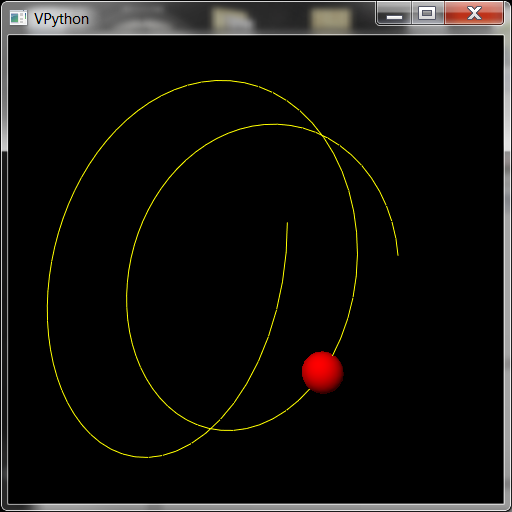
\includegraphics[width=\textwidth]{images/vpythonpcurve.png}
\column{0.5\textwidth}
\[
f(t) = (10\cos(t), 10\sin(t), t)
\]
\end{columns}
\end{frame}

\sect{Parametric Curves: Tangent, Normal, Binormal}
\begin{columns}[c]
\column{0.5\textwidth}
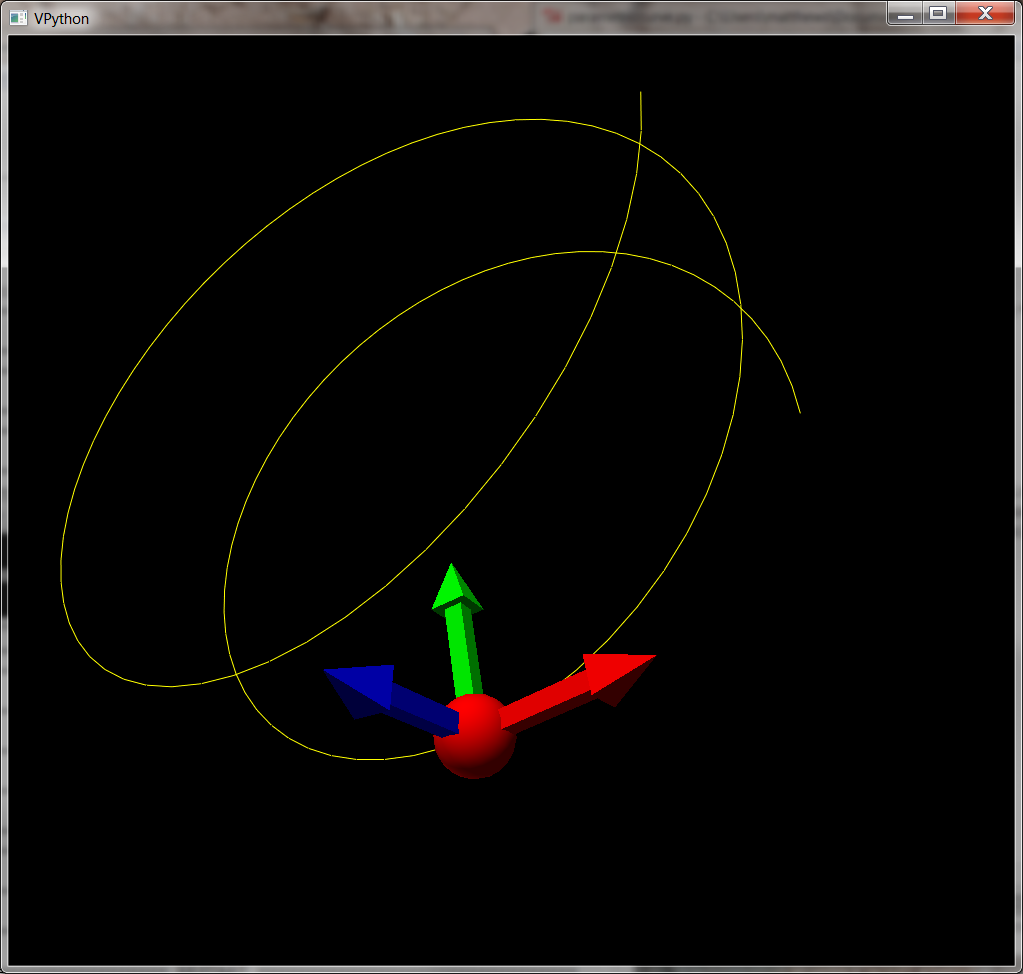
\includegraphics[width=\textwidth]{images/vpythoncurveframe.png}
\column{0.5\textwidth}
\begin{eqnarray*}
f(t) &=& (10\cos(t), 10\sin(t), t)\\
\frac{df}{dt} &=& (-10\sin(t), 10\cos(t), 1)\\
\frac{d^2f}{dt^2} &=& (-10\cos(t), -10\sin(t), 0)
\end{eqnarray*}
\begin{eqnarray*}
\frac{df}{dt}\times \frac{d^2f}{dt^2} &\propto& (\sin(t), \cos(t), 10)
\end{eqnarray*}
\end{columns}
\end{frame}

\sect{Parametric Surfaces}
\begin{columns}[c]
\column{0.5\textwidth}
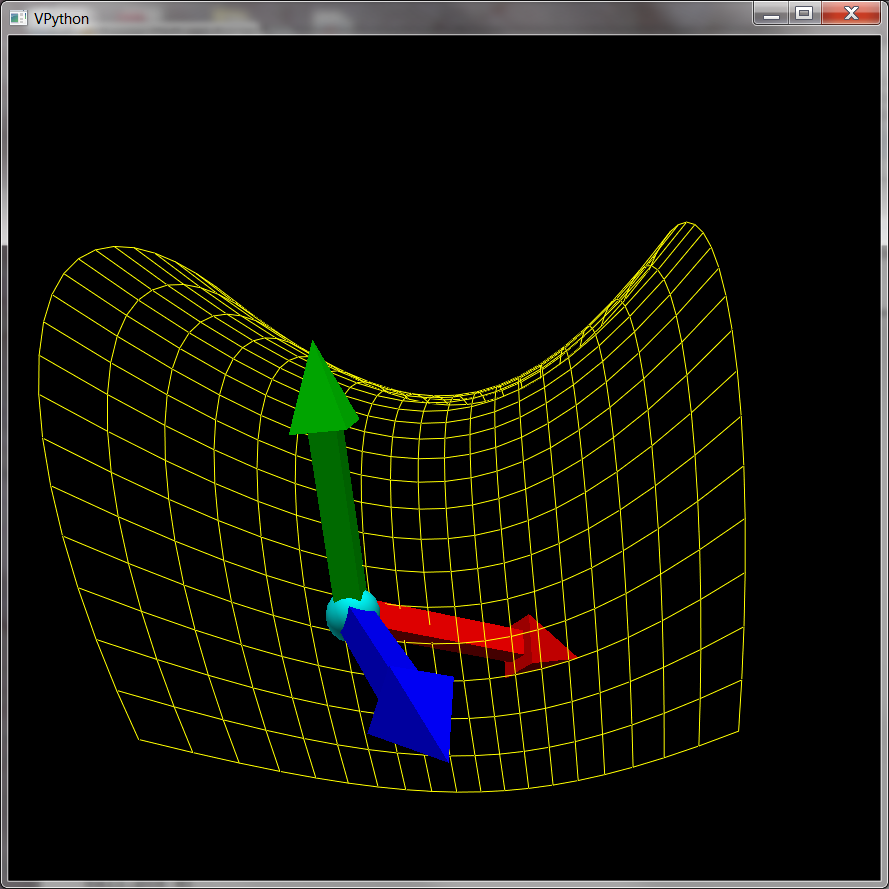
\includegraphics[width=\textwidth]{images/vpythonpsurface.png}
\column{0.5\textwidth}
Explicit:
\[
f(s,t) = (s, t, s^2-t^2)
\]
Implicit:
\begin{eqnarray*}
F(x,y,z) &=& 0\\\pause
x^2 - y^2 &=& z\\\pause
x^2 - y^2 - z &=& 0
\end{eqnarray*}
\end{columns}
\end{frame}

\sect{Parametric Surfaces: Normal, Tangent, Binormal}
\begin{columns}[c]
\column{0.5\textwidth}
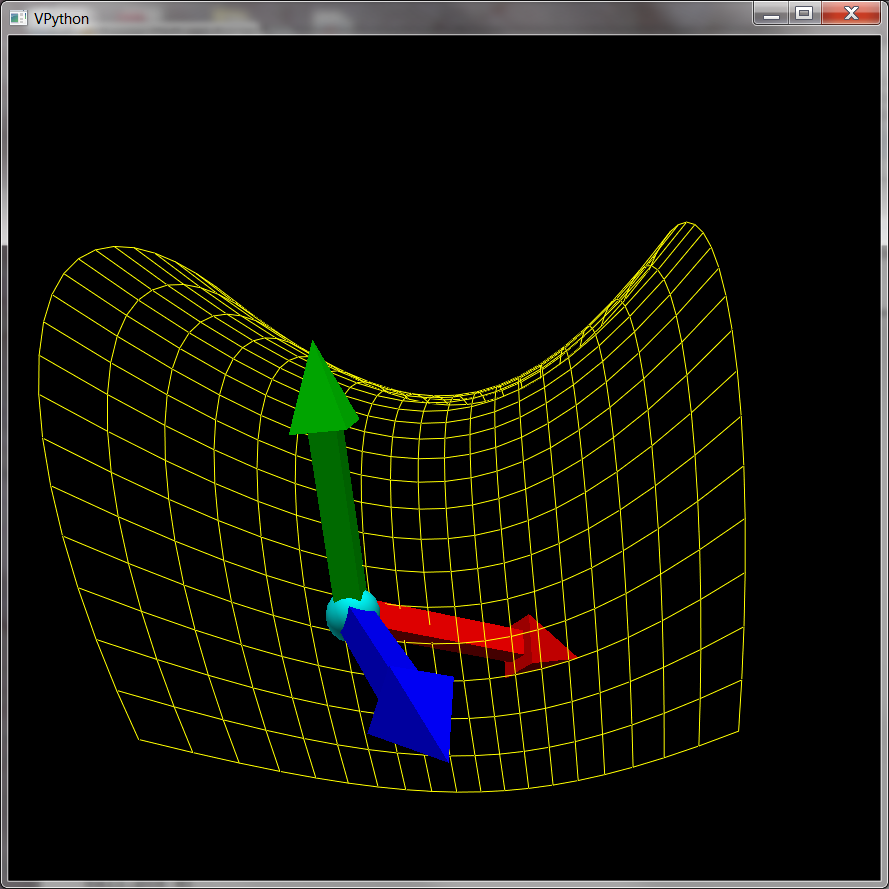
\includegraphics[width=\textwidth]{images/vpythonpsurface.png}
\column{0.5\textwidth}
\begin{eqnarray*}
f(s,t) &=& (s, t, s^2-t^2)\\
\frac{\partial f}{\partial s} &=& (1, 0, 2s)\\
\frac{\partial f}{\partial t} &=& (0, 1, -2t)\\
\frac{\partial f}{\partial s} \times
\frac{\partial f}{\partial t} &=& (-2s, 2t, 1)
\end{eqnarray*}
\begin{eqnarray*}
F(x,y,z) &=& x^2 - y^2 - z\\
\nabla F(x,y,z) &=& (2x, -2y, -1)
\end{eqnarray*}
\end{columns}
\end{frame}

\sect{Parametric Surfaces: Sphere}
\begin{columns}[c]
\column{0.5\textwidth}
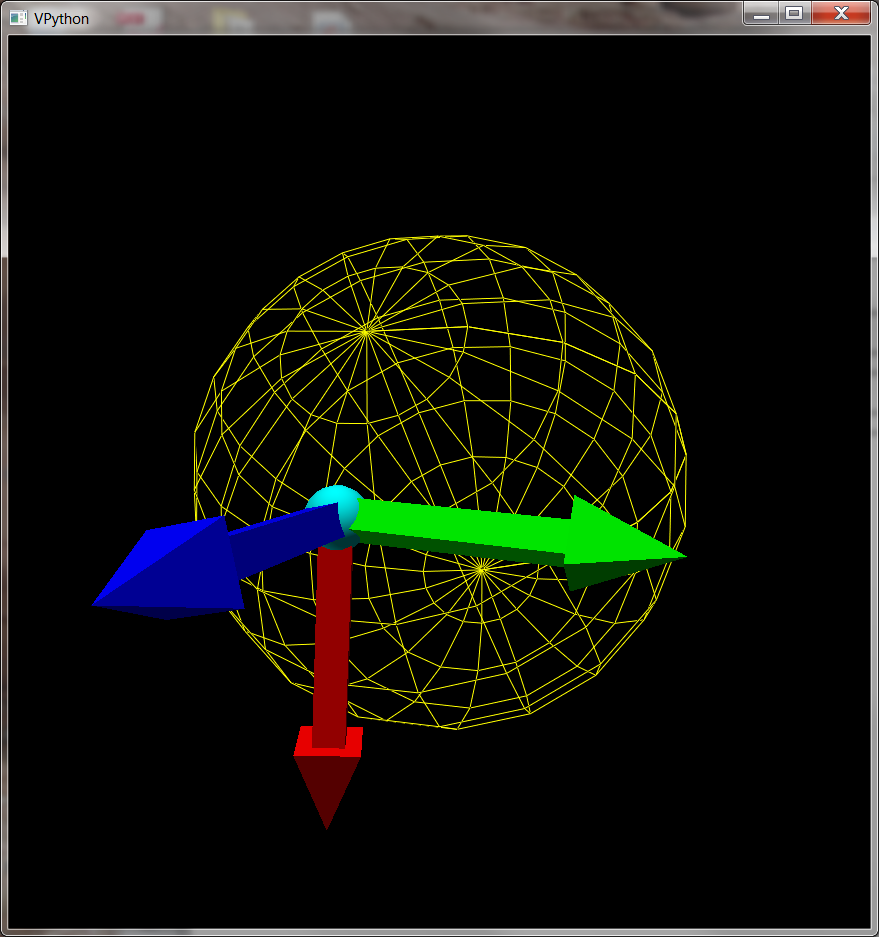
\includegraphics[width=\textwidth]{images/vpythonpsphere.png}
\column{0.5\textwidth}
Explicit:
\begin{eqnarray*}
f(s,t) &=& (\cos(t)\cos(s),\\&&\cos(t)\sin(s),\\&&\sin(t))
\end{eqnarray*}
Implicit:
\begin{eqnarray*}
x^2 + y^2 + z^2 &=& 1\\
x^2 + y^2 + z^2 - 1 &=& 0
\end{eqnarray*}
\end{columns}
\end{frame}

\sect{Parametric Surfaces: Normal, Tangent, Binormal}
\begin{columns}[c]
\column{0.4\textwidth}
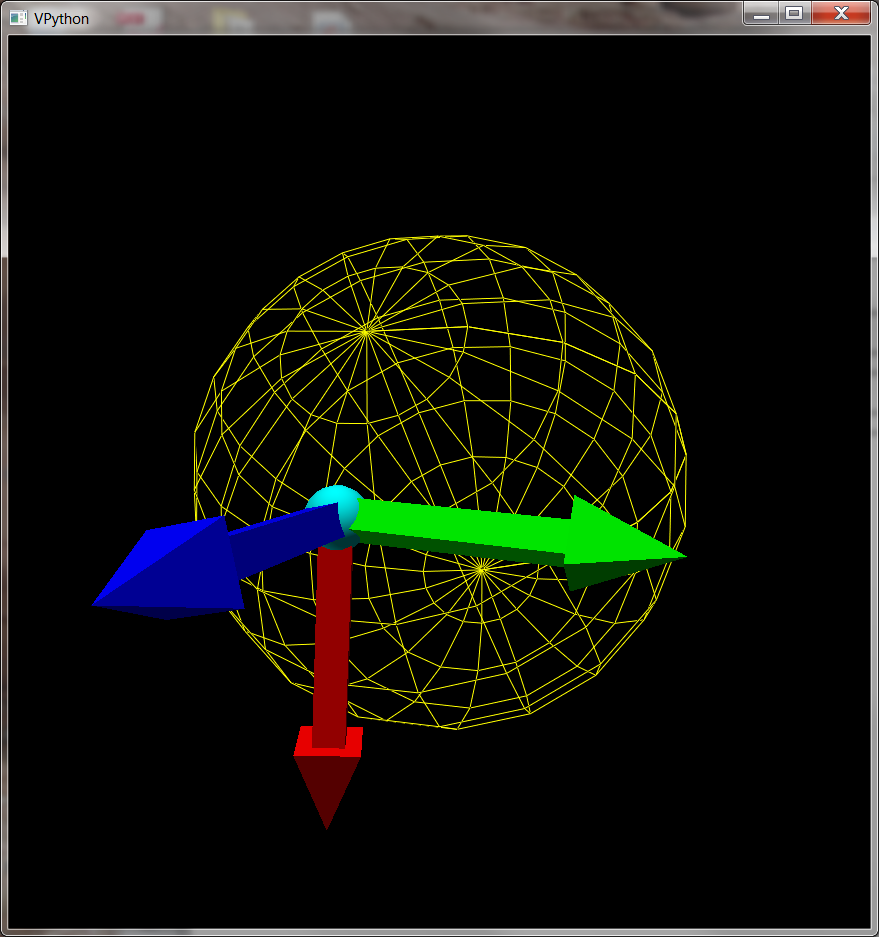
\includegraphics[width=\textwidth]{images/vpythonpsphere.png}
\column{0.6\textwidth}
\begin{eqnarray*}
F(x,y,z) &=& x^2 + y^2 + z^2 - 1 \\
\nabla F(x,y,z) &=& (2x, 2y, 2z)
\end{eqnarray*}
\end{columns}
\begin{eqnarray*}
f(s,t) &=& (\cos(t)\cos(s),\cos(t)\sin(s),\sin(t))\\
\frac{\partial f}{\partial s} &=& (-\cos(t)\sin(s),
                                   \cos(t)\cos(s),
                                   0)\\
\frac{\partial f}{\partial t} &=& (-\sin(t)\cos(s),
                                   -\sin(t)\sin(s),
                                    \cos(t))\\
\end{eqnarray*}
\end{frame}

\sect{Approximations to Tangent, Normal, Binormal}
\begin{eqnarray*}
\frac{\partial f}{\partial s} &\approx\propto&
\frac{f(s+\epsilon, t) - f(s,t)}{|f(s+\epsilon, t) - f(s,t)|}\\
\frac{\partial f}{\partial t} &\approx\propto&
\frac{f(s, t+\epsilon) - f(s,t)}{|f(s, t+\epsilon) - f(s,t)|}\\
\mbox{\it Normal} &=& \frac{\partial f}{\partial s} \times \frac{\partial f}{\partial g}
\end{eqnarray*}
\end{frame}


\sect{Quadrics}
\newcommand{\qg}[1]{\includegraphics[scale=0.25]{images/#1}}
\url{http://tutorial.math.lamar.edu/Classes/CalcIII/QuadricSurfaces.aspx}

\qg{cone.png}\hfill
\qg{ellipsoid.png}\hfill
\qg{ellipticparaboloid.png}

\qg{hyperbolicparaboloid.png}\hfill
\qg{hyperboloidofonesheet.png}\hfill
\qg{hyperboloidoftwosheets.png}
\end{frame}

\newcommand{\quadric}[1]{
\includegraphics[scale=0.5]{images/#1}
}

\sect{Ellipsoid}
 $x^2+y^2+z^2-1$ \hfill
 $(\cos(v)\cos(u),\cos(v)\sin(u),\sin(v))$ \\
\hfill $v\in[-\pi/2,\pi/2], u\in[-\pi,\pi]$

\quadric{ellipsoid.png}

\vfill

Equations from {\em Computer Graphics Using Open GL, 2E}
\end{frame}
\sect{Hyperboloid of one sheet}
 $x^2+y^2-z^2-1$\hfill
$(\sec(v)\cos(u),\sec(v)\sin(u),\tan(v))$\\
\hfill$v\in[-\pi/2,\pi/2], u\in[-\pi,\pi]$

\quadric{hyperboloidofonesheet.png}
\end{frame}

\sect{Hyperboloid of two sheets}
 $x^2-y^2-z^2-1$\hfill
$(\sec(v)\cos(u),\sec(v)\tan(u),\tan(v))$\\
\hfill$v\in[-\pi/2,\pi/2],[\pi/2,3\pi/2], u\in[-\pi,\pi]$\\
\hfill {\large \bf ?}

\quadric{hyperboloidoftwosheets.png}
\end{frame}

\sect{Elliptic cone}
 $x^2+y^2-z^2$\hfill
$(v\cos(u),v\sin(u),v)$\\
\hfill $v\in[-\infty,+\infty],u\in[-\pi,\pi]$\\

\quadric{cone.png}
\end{frame}

\sect{Elliptic paraboloid}

 $x^2+y^2-z$\hfill
$(v\cos(u),v\sin(u),v^2)$\\
\hfill $v\in[0,+\infty],u\in[-\pi,\pi]$\\
\quadric{ellipticparaboloid}
\end{frame}

\sect{Hyperbolic paraboloid}
 $-x^2+y^2-z$\hfill
$(v\tan(u),v\sec(u),v^2)$\\
\hfill$v\in[0,+\infty],u\in[-\pi,\pi]$\\
\quadric{hyperbolicparaboloid.png}
\end{frame}

\sect{Surfaces of Revolution}
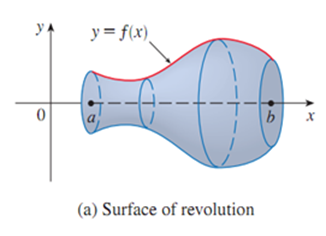
\includegraphics[scale=0.75]{images/sor.png}\hfill
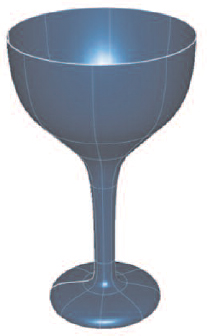
\includegraphics[scale=0.4]{images/sorcup.jpg}

If $y=f(x)$ is determined by a series of points $(x_0,y_0),\ldots(x_n,y_n)$,
then let $s\in[0,\ldots, n]$ and $t\in[0,2\pi]$, and the parametric
surface is
\[
(x_s, y_s\cos(t),  y_s\sin(t))
\]
\end{frame}

\sect{Tubes along 3D curves}

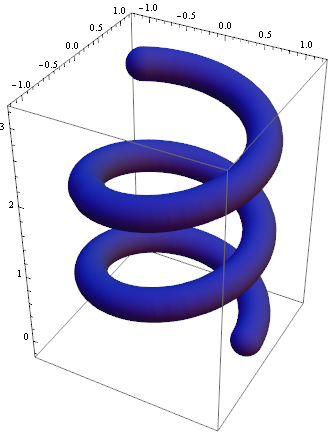
\includegraphics[width=0.3\textwidth]{images/extrudedtube.png}
\hfill
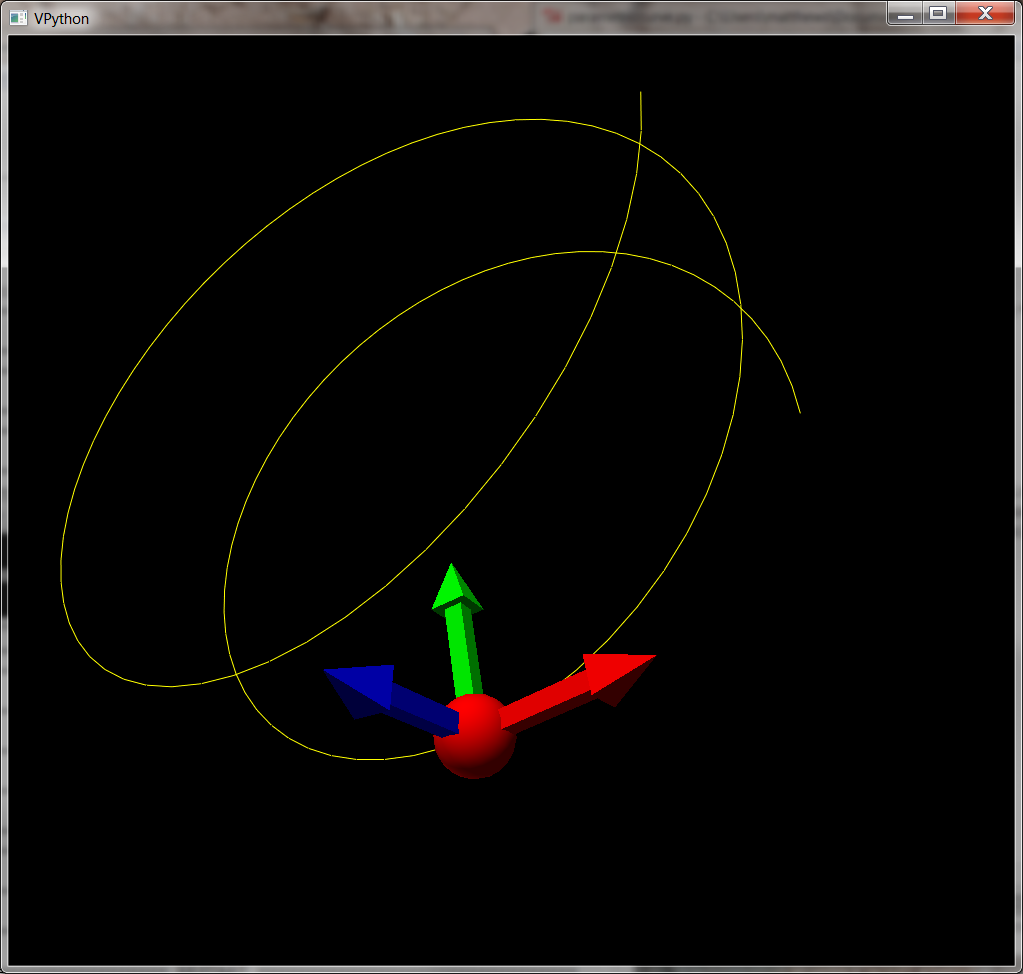
\includegraphics[width=0.4\textwidth]{images/vpythoncurveframe.png}

\begin{itemize}
\item Assume the curve is parameterized by $f(s)$, $s\in[a,b]$
\item Find the tangent, normal, and binormal to the curve: $t,n,b$
\item The parametric surface, parameterized by $s\in[a,b]$, $t\in[0,2\pi]$:
\[
f(s) + \cos(t)n + \sin(t)b
\]
\item Could you extrude an arbitrary shape instead of a circle?
\end{itemize}

\end{frame}


\end{document}
